\chapter{सर्वसम कण}\label{ch:b3:identical-particles}

ब्रह्मांड का हर इलेक्ट्रॉन हर दूसरे इलेक्ट्रॉन के ठीक-ठीक, पूर्णतः
सर्वसम है --- एक टकसाल के दो सिक्कों की तरह मिलता-जुलता नहीं, बल्कि
सैद्धांतिक रूप से अभेद्य: न कोई नामपत्र, न खरोंच, न इतिहास किसी एक को
चिह्नित कर सकता है। क्वांटम यांत्रिकी इसे गंभीरता से लेती है, और उसके
परिणाम संसार चलाते हैं। दो सर्वसम कणों की अदला-बदली से कोई भी प्रेक्ष्य
वस्तु बदलनी नहीं चाहिए, और इससे बहु-कण तरंग फलन के पास केवल दो विकल्प
बचते हैं: वही रहे (\emph{बोसॉन}) या चिह्न बदल ले (\emph{फ़र्मिऑन})।
अकेले उस ऋण चिह्न से \omterm{cor:b3:identical-particles:pauli}{पाउली का अपवर्जन सिद्धांत} निकलता है, कोश-संरचना
और पूरी \omterm{prop:b3:identical-particles:periodic}{आवर्त सारणी}, पैरों तले पदार्थ की कठोरता, और वह दाब जो मरे हुए
तारों को थामे रखता है; और धन चिह्न से फ़ोटॉनों की मिलनसारी --- अर्थात्
लेज़र --- तथा तीन अध्याय आगे, बोस--आइंस्टाइन संघनन। भौतिकी में शायद ही
कभी एक चिह्न ने इतना बोझ ढोया हो।

\section{सममितीकरण अभिगृहीत}

\begin{definition}[विनिमय]\label{def:b3:identical-particles:exchange}
\index{सर्वसम कण}\index{विनिमय संकारक}
दो सर्वसम कणों के लिए, जिनका अवस्था-समष्टि गुणनफलों
$\ket{a}\otimes\ket{b}$ से फैला है (कण 1 $\ket a$ में, कण 2
$\ket b$ में --- स्थितियाँ, चक्रण और सब कुछ), \emph{विनिमय संकारक}
$\hat P_{12}$ भूमिकाएँ अदल-बदल देता है: $\hat P_{12}\ket a\otimes\ket b =
\ket b\otimes\ket a$। यह हर्मिटीय है, इसका वर्ग तत्समक है, और यह हर उस
हैमिल्टनियन से क्रमविनिमेय है जो कणों को सर्वसम मानता है:
उसके \omterm{def:b3:quantum-formalism:observable}{अभिलक्षणिक मान} $\pm1$ संसार के संरक्षित नामपत्र हैं।
\end{definition}

\begin{theorem}[बोसॉन और फ़र्मिऑन]\label{thm:b3:identical-particles:postulate}
\index{बोसॉन}\index{फ़र्मिऑन}\index{चक्रण-सांख्यिकी प्रमेय}
सर्वसम कणों की अवस्थाएँ हर विनिमय की अभिलक्षणिक अवस्थाएँ होने के लिए
केवल अनुमत नहीं, बल्कि \emph{बाध्य} हैं: कणों के एक वर्ग के लिए पूर्णतः
\emph{सममित} --- अर्थात् \emph{बोसॉन} --- और दूसरे के लिए पूर्णतः
\emph{प्रतिसममित} (हर अदला-बदली पर चिह्न-परिवर्तन) --- अर्थात्
\emph{फ़र्मिऑन}। कोई जाति किस वर्ग की है, यह उसका चक्रण तय करता है
(\emph{चक्रण--सांख्यिकी प्रमेय}, जो केवल आपेक्षिकीय क्वांटम क्षेत्र
सिद्धांत में सिद्ध होती है और यहाँ मान ली गई है):
\[
\text{पूर्णांक चक्रण} \Rightarrow \text{बोसॉन} , \qquad
\text{अर्ध-पूर्णांक चक्रण} \Rightarrow \text{फ़र्मिऑन} .
\]
फ़ोटॉन, पायॉन और $^4$He परमाणु बोसॉन हैं; इलेक्ट्रॉन, प्रोटॉन,
न्यूट्रॉन और $^3$He फ़र्मिऑन हैं।
कोई संयुक्त कण अपने अंगों के योग जैसा बरतता है: एक साथ बँधे फ़र्मिऑनों
की सम संख्या एक बोसॉन है ($^4$He: 2p + 2n + 2e), और विषम संख्या एक
फ़र्मिऑन ($^3$He) --- ऐसे परिणामों के साथ, जो दो अलग-अलग द्रव
हीलियमों जितने दृश्य हैं।
\end{theorem}
\admitted

\begin{corollary}[पाउली का अपवर्जन सिद्धांत]\label{cor:b3:identical-particles:pauli}
\index{पाउली का अपवर्जन सिद्धांत}
दो फ़र्मिऑन कभी एक ही एक-कण अवस्था नहीं घेर सकते: प्रतिसममित संयोजन में
$\ket a = \ket b$ रखिए, अर्थात्
$(\ket a\otimes\ket b - \ket b\otimes\ket a)/\sqrt2$, और शून्य सदिश
मिलता है --- ऐसी कोई अवस्था है ही नहीं। इलेक्ट्रॉनों (चक्रण $\tfrac12$)
के लिए हर कक्षक अधिक से अधिक दो को लेता है, विपरीत चक्रण-प्रक्षेप वाले।
\end{corollary}

\begin{example}[अलग ढंग की गणना]\label{ex:b3:identical-particles:counting}
दो अवस्थाओं $a, b$ में दो कण: चिरसम्मत (विभेद्य) गणना चार विन्यास देती
है; बोसॉनों के पास तीन हैं ($aa$, $bb$, और \emph{एक} मिश्रित अवस्था);
फ़र्मिऑनों के पास ठीक एक (वही मिश्रित, प्रतिसममित वाली)। सांख्यिकीय
भौतिकी इन्हीं गणनाओं को जस का तस उत्तराधिकार में लेगी
(\cref{ch:b3:quantum-statistics}); और यहीं वे उन्नीसवीं सदी की एक
लज्जा घोल देती हैं --- एक ही गैस के दो नमूनों के ``मिश्रण'' की
एन्ट्रॉपी (\cref{exo:b3:identical-particles:10})।
\end{example}

\section{आवर्त सारणी}

\begin{proposition}[कोश, और रसायन क्यों है]\label{prop:b3:identical-particles:periodic}
\index{आवर्त सारणी}\index{आउफ़बाउ सिद्धांत}
हाइड्रोजन-सदृश कक्षकों $(n, l, m, m_s)$ को एक-एक इलेक्ट्रॉन से भरिए,
पहले सबसे कम ऊर्जा वाले, उस स्तर-क्रम में जो भेदन और परिरक्षण तय करते
हैं ($1s$, $2s$, $2p$, $3s$, $3p$, $4s$, $3d$, \dots ---
\cref{exo:b3:hydrogen-atom:8})। पाउली का सिद्धांत भरने को
\emph{संतृप्त} कर देता है: $2$ इलेक्ट्रॉन पहला कोश बंद करते हैं, $8$
दूसरी और तीसरी पंक्ति, और तत्त्वों की सारणी को उसके आवर्त मिल जाते
हैं। रसायन उन्हीं इलेक्ट्रॉनों की भौतिकी है जिन्हें अपवर्जन सिद्धांत ने
सबसे बाहर छोड़ दिया: भरे हुए कोश (उत्कृष्ट गैसें) निष्क्रिय हैं; भरे
कोश से एक इलेक्ट्रॉन आगे (क्षार धातुएँ) या एक विवर पीछे (हैलोजन)
विपरीत ढंगों से क्रियाशील हैं। ऋण चिह्न के बिना हर इलेक्ट्रॉन $1s$ में
डूब जाता, हर परमाणु सिकुड़ी हुई हीलियम-सी गेंद होता, और न कोई बंध
होता, न अणु, न पछताने के लिए कोई रसायनज्ञ।
\end{proposition}
\admitted

\begin{omfigure}
\begin{tikzpicture}[font=\small, >=Stealth]
  % 1s
  \draw[thick] (0,0) rectangle (1.0,0.7);
  \node[anchor=north] at (0.5,-0.08) {$1s$};
  \node at (0.5,0.35) {$\uparrow\downarrow$};
  % 2s
  \draw[thick] (1.9,0) rectangle (2.9,0.7);
  \node[anchor=north] at (2.4,-0.08) {$2s$};
  \node at (2.4,0.35) {$\uparrow\downarrow$};
  % 2p: three boxes
  \foreach \i in {0,1,2} \draw[thick] ({3.5+\i*1.05},0) rectangle ({4.5+\i*1.05},0.7);
  \node[anchor=north] at (5.05,-0.08) {$2p$ (तीन कक्षक)};
  \node at (4.0,0.35) {$\uparrow\downarrow$};
  \node at (5.05,0.35) {$\uparrow$};
  \node at (6.1,0.35) {$\uparrow$};
  \node[anchor=west, align=left, font=\footnotesize] at (7.4,0.35)
    {ऑक्सीजन ($Z = 8$): $1s^2\,2s^2\,2p^4$\\
     समांतर चक्रण पहले फैलते हैं\\ (हुंड का नियम)};
  \draw[decorate, decoration={brace, mirror, amplitude=4pt}] (0,-0.65) -- (2.9,-0.65);
  \node[font=\footnotesize] at (1.45,-1.05) {He, Be पर बंद};
  \draw[decorate, decoration={brace, mirror, amplitude=4pt}] (3.5,-0.65) -- (6.55,-0.65);
  \node[font=\footnotesize] at (5.05,-1.05) {Ne पर बंद: रसायन समाप्त};
\end{tikzpicture}

{\small कक्षकों को दो-दो करके भरना: अपवर्जन सिद्धांत सारणी के आवर्त
गढ़ता है। ऑक्सीजन के चार $2p$ इलेक्ट्रॉन हुंड का नियम दिखाते हैं ---
चक्रण जोड़ा बनाने से पहले संरेखित होकर कक्षकों में फैल जाते हैं,
जो विशुद्ध विनिमय-प्रभाव है
(\cref{prop:b3:identical-particles:exchange-force}).}
\end{omfigure}

\section{विनिमय अन्योन्यक्रिया}

\begin{proposition}[स्थानिक युग्म-अवस्था की सममिति]\label{prop:b3:identical-particles:exchange-force}
\index{विनिमय अन्योन्यक्रिया}
दो इलेक्ट्रॉनों के लिए कुल अवस्था (समष्टि $\times$ चक्रण) प्रतिसममित
होनी चाहिए: कोई \emph{एकल} (प्रतिसममित चक्रण,
\cref{exo:b3:spin-two-level:11}) स्थानिक तरंग फलन को \emph{सममित} होने
पर बाध्य करता है, और कोई \emph{त्रिक} उसे प्रतिसममित। दोनों भौतिक रूप
से भिन्न हैं: प्रतिसममित स्थानिक अवस्था में इलेक्ट्रॉन कभी संपाती नहीं
हो सकते ($\psi(\vect r, \vect r) = 0$) और दूर-दूर रहते हैं, जबकि
सममित अवस्था उन्हें गुच्छा बनाने देती है। चूँकि निकटता कूलॉम ऊर्जा
वसूलती है, चक्रण-विन्यास को एक ऊर्जा-अंतर मिल जाता है --- \emph{विनिमय
ऊर्जा} --- जो स्थिरवैद्युत आकार का है (इलेक्ट्रॉन-वोल्ट!), जबकि उतना
प्रबल कोई चुंबकीय बल है ही नहीं: चक्रण ज्यामिति और प्रतिकर्षण के कारण
संरेखित या प्रति-संरेखित होते हैं। यही हुंड के नियम का, हीलियम के दो
वर्णक्रमों का, सहसंयोजी बंध का और --- किसी क्रिस्टल भर में बढ़ाकर ---
स्वयं लौहचुंबकत्व का इंजन है
(\cref{ch:b3:electromagnetism-in-matter})।
\end{proposition}

\begin{proof}[आंशिक उपपत्ति]
सममिति का हिसाब \cref{thm:b3:identical-particles:postulate} और
चक्रण-संयोजन हैं; और संपात पर लुप्त होना $\vect r_1 = \vect r_2$ पर
पढ़ी गई प्रतिसममिति है। ऊर्जा-परिणाम प्रतिकर्षण में प्रथम-कोटि
\omterm{thm:b3:perturbation-theory:corrections}{विक्षोभ सिद्धांत} है: सीधा पद दोनों सममितियों में उभयनिष्ठ है, और
आड़ा (``विनिमय'') समाकल विपरीत चिह्नों के साथ आता है
(\cref{exo:b3:identical-particles:6})।
\end{proof}

\begin{omfigure}
\begin{tikzpicture}
  \begin{axis}[omaxis, axis x line=bottom, axis y line=left,
    width=11.4cm, height=5.4cm, xmin=-3.4, xmax=3.4, ymin=0, ymax=1.28,
    xlabel={पृथक्करण $x_1 - x_2$ (स्वेच्छ इकाइयाँ)},
    ylabel={युग्म घनत्व},
    xlabel style={at={(axis description cs:0.5,-0.1)}, anchor=north},
    xtick=\empty, ytick=\empty, clip=false,
    legend style={font=\scriptsize, at={(0.98,0.76)}, anchor=north east,
      draw=none, fill=none}]
    \addplot[omThm, very thick, domain=-3.4:3.4, samples=120]
      {(1+exp(-x*x))*exp(-x*x/6)*0.62};
    \addlegendentry{सममित (बोसॉन; एकल इलेक्ट्रॉन)}
    \addplot[omDef, very thick, domain=-3.4:3.4, samples=120]
      {(1-exp(-x*x))*exp(-x*x/6)*0.9};
    \addlegendentry{प्रतिसममित (त्रिक इलेक्ट्रॉन)}
  \end{axis}
\end{tikzpicture}

{\small युग्म को पृथक्करण $x_1 - x_2$ पर पाने की प्रायिकता:
सममित स्थानिक अवस्था संपर्क पर गुच्छा बनाती है, और प्रतिसममित अवस्था
एक ``विनिमय विवर'' ढोती है --- संपात पर ठीक शून्य। इस ज्यामिति को
कूलॉम प्रतिकर्षण को खिलाइए, और चक्रण-विन्यासों को इलेक्ट्रॉन-वोल्ट के
ऊर्जा-अंतर मिल जाते हैं।}
\end{omfigure}

\begin{example}[एक ही परमाणु में दो हीलियम]\label{ex:b3:identical-particles:helium}
हीलियम की उत्तेजित अवस्थाएँ $1s\,2s$ दो कुलों में आती हैं, जो शायद ही
आपस में मिलती हैं: \emph{पैरा}हीलियम (एकल, सममित समष्टि) और
\emph{ऑर्थो}हीलियम (त्रिक, प्रतिसममित समष्टि), जिनमें त्रिक
$\approx\qty{0.8}{eV}$ \emph{नीचे} पड़ता है --- उसका विनिमय विवर
कूलॉम प्रतिकर्षण बचा देता है। मूल अवस्था अनिवार्यतः पैरा है ($1s^2$
सममित स्थानिक अवस्था थोपता है); और सबसे नीची ऑर्थो अवस्था, जिसके नीचे
क्षय के लिए कोई त्रिक नहीं और जिसके चक्रण-पलटाव वर्जित हैं, घंटों
जीती है --- एक अर्धस्थायी परमाणु, जो परमाणु-पुंजों में मज़दूर की तरह
काम आता है। उन्नीसवीं सदी के वर्णक्रममितिज्ञों ने ``दो हीलियम''
सूचीबद्ध किए थे; समाधान एक ऋण चिह्न है।
\end{example}

\begin{example}[सहसंयोजी बंध]\label{ex:b3:identical-particles:bond}
दो हाइड्रोजन परमाणुओं को पास लाइए: दोनों इलेक्ट्रॉन दो परमाणविक कक्षकों
का सममित स्थानिक संयोजन (चक्रण एकल) या प्रतिसममित संयोजन (त्रिक) चुन
सकते हैं। सममित अवस्था आवेश को प्रोटॉनों के \emph{बीच} ढेर कर देती है,
जहाँ वह दोनों को खींचता है: अर्थात् बंधन --- H$_2$ का सहसंयोजी बंध,
\qty{4.5}{eV} गहरा। प्रतिसममित अवस्था मध्य-तल खाली कर देती है: विशुद्ध
प्रतिकर्षी। कार्बनिक रसायन की हर पंक्ति सममित रूप से साझा किए गए
युग्मित-चक्रण इलेक्ट्रॉनों का हिसाब है --- अपवर्जन सिद्धांत, उलटा
चलाकर, अणुओं का गोंद है।
\end{example}

\section{बोसॉन: जितने अधिक, उतना अच्छा}

\begin{proposition}[बोसॉनी संवर्धन]\label{prop:b3:identical-particles:enhancement}
\index{उद्दीपित उत्सर्जन!बोसॉनी उद्गम}
जो संक्रमण किसी ऐसी अवस्था में एक बोसॉन जोड़ते हैं जिसमें पहले से $n$
हैं, उनके आयाम $\sqrt{n + 1}$ से और दरें $n + 1$ से बढ़ जाती हैं
(\cref{ch:b3:harmonic-oscillator} का सोपान बीजगणित, चूँकि कोई बोसॉनी
मोड दोलक \emph{होता} ही है)। वह ``$1$'' स्वतःस्फूर्त उत्सर्जन है; और
वह ``$n$'' \emph{उद्दीपित} उत्सर्जन, जो पहले से मौजूद भीड़ के
अनुक्रमानुपाती है: हर लेज़र के पीछे का हिमस्खलन (वर्ष 2 का खंड), जो अब
विशुद्ध विनिमय-सममिति निकला। यही सांख्यिकी, तब तक ठंडे किए गए परमाणुओं
पर लागू करने पर जब तक उनके तरंग-पुंज अतिव्यापी न हो जाएँ, एक ही
क्वांटम अवस्था में भगदड़ की भविष्यवाणी करती है --- बोस--आइंस्टाइन
संघनन, जो \cref{ch:b3:quantum-statistics} के लिए रखा है।
\end{proposition}
\admitted

\begin{method}[सर्वसम कणों को बरतना]\label{met:b3:identical-particles:method}
(1) चक्रण से सांख्यिकी तय कीजिए (संयुक्त कणों में फ़र्मिऑनों की संख्या
जोड़िए)। (2) दो इलेक्ट्रॉनों के लिए समष्टि $\times$ चक्रण में
गुणनखंडित कीजिए, और एकल को सममित समष्टि से तथा त्रिक को प्रतिसममित से
जोड़िए। (3) अवस्थाएँ गिनिए, नाम वाले कण कभी नहीं: अधिभोग सूचीबद्ध
कीजिए। (4) प्रतिकर्षण वाले ऊर्जा-प्रश्न: सीधा समाकल एक बार, और विनिमय
समाकल सममिति के चिह्न के साथ। (5) दो सूत्र याद रखिए --- फ़र्मिऑन: प्रति
अवस्था अधिक से अधिक एक, और हर एक के चारों ओर एक विनिमय विवर; बोसॉन:
अधिभोग से बढ़ी हुई दरें।
\end{method}

\begin{omfigure}
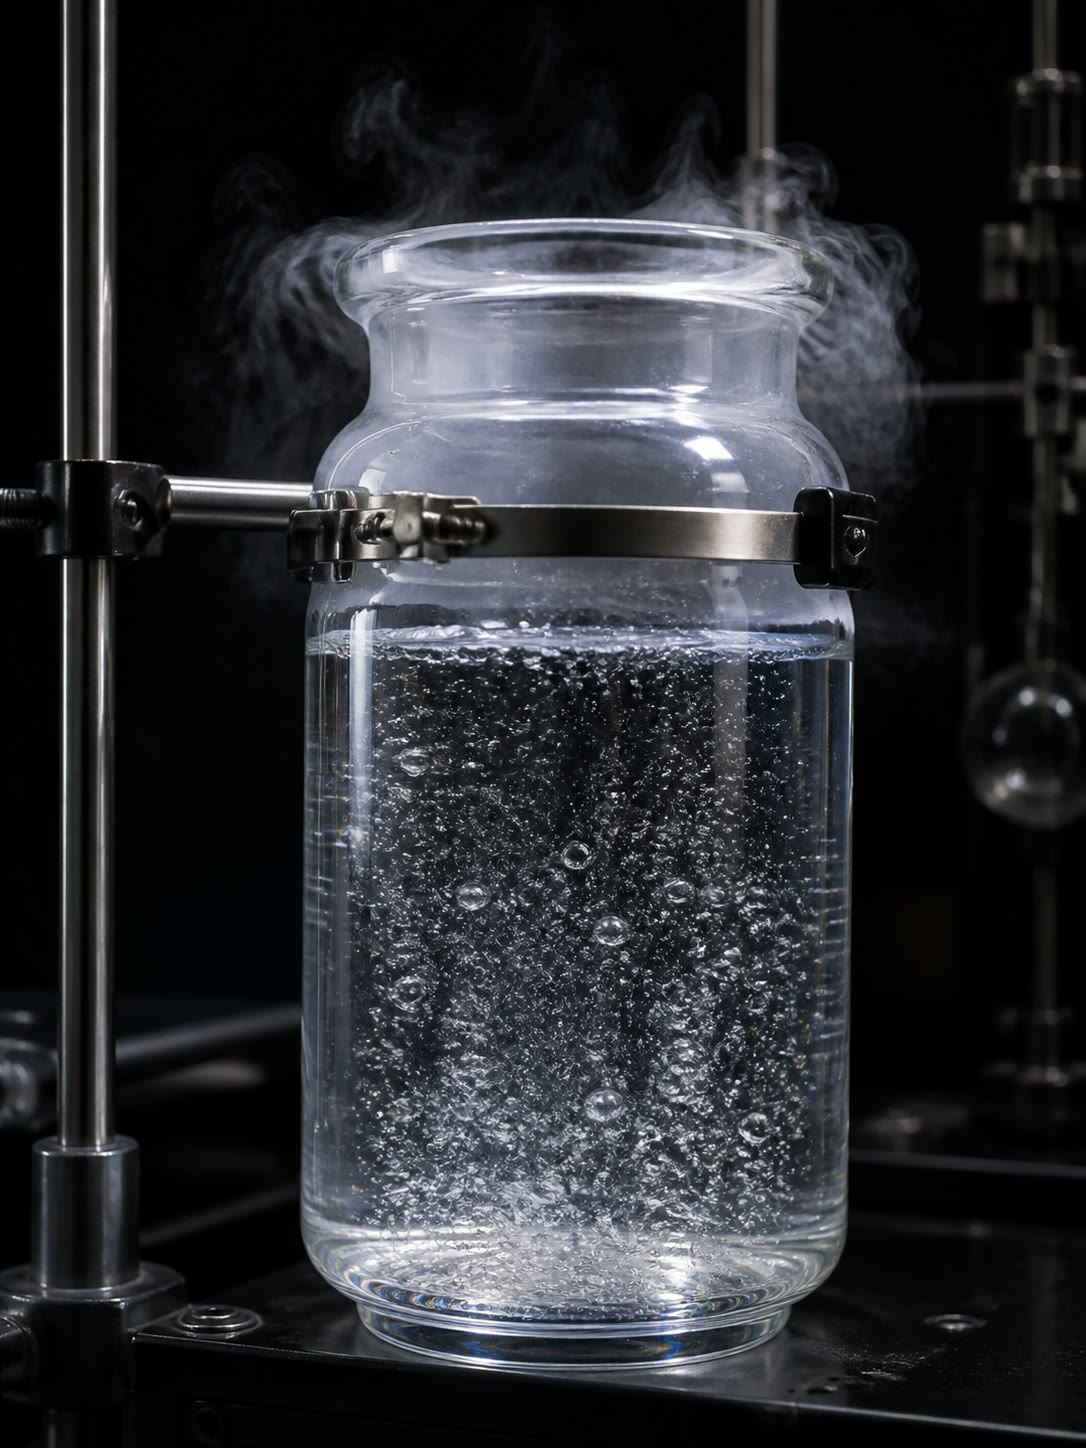
\includegraphics[width=0.45\linewidth]{images/book5/ai/b5-14-liquid-helium-dewar.jpg}

{\small द्रव हीलियम, \qty{4}{K} के पास चुपचाप उबलता हुआ: पूर्णतः सर्वसम बोसॉनों का एक तरल। कुछ ही डिग्री नीचे वह अचानक उबलना बंद कर देता है और बिना घर्षण बहने लगता है --- अभेद्यता, जो द्रवचालिकी तक पदोन्नत हो गई।}
\end{omfigure}

\section{अभ्यास}

\begin{exercise}[$\star$]\label{exo:b3:identical-particles:1}
(क) दिखाइए कि $\hat P_{12}$ हर्मिटीय है और $\hat P_{12}^2 = \mathbb 1$:
उसके संभव \omterm{def:b3:quantum-formalism:observable}{अभिलक्षणिक मान} क्या हैं? (ख) सर्वसम कणों के लिए दिखाइए कि $[\hat P_{12}, \hat H] =
0$ और निष्कर्ष निकालिए कि सममिति-वर्ग संरक्षित है। (ग) दो सर्वसम कणों
की कोई अवस्था बिना किसी सममिति के बस $\ket a\otimes\ket b$ क्यों नहीं
``हो'' सकती? (घ) वर्गीकृत कीजिए:
$^1$H, $^2$H (ड्यूटीरियम), $^4$He, $^3$He, एक हाइड्रोजन अणु, एक
फ़ोटॉन।
\end{exercise}

\begin{exercise}[$\star$]\label{exo:b3:identical-particles:2}
(क) लांबिक कक्षकों $\ket a, \ket b$ से बनी प्रसामान्यित प्रतिसममित
अवस्था लिखिए। (ख) दिखाइए कि $a = b$ होने पर वह लुप्त हो जाती है। (ग)
$a, b, c$ में तीन फ़र्मिऑनों के लिए: पूर्णतः प्रतिसममित संयोजन लिखिए
(छह पद, बदलते चिह्न --- एक $3\times3$ सारणिक) और जाँचिए कि एक
अदला-बदली उसका चिह्न पलट देती है। (घ) सारणिक-रूप पाउली के सिद्धांत को
स्वतः क्यों बना देता है?
\end{exercise}

\begin{exercise}[$\star$]\label{exo:b3:identical-particles:3}
दो कण तीन लांबिक अवस्थाएँ साझा करते हैं। दो-कण अवस्थाएँ गिनिए: (क)
विभेद्य कणों के लिए; (ख) बोसॉनों के लिए; (ग) फ़र्मिऑनों के लिए
(चक्रणहीन)। (घ) चक्रण वाले इलेक्ट्रॉनों के लिए (ग) दोहराइए: अब कितनी
अवस्थाएँ?
\end{exercise}

\begin{exercise}[$\star$]\label{exo:b3:identical-particles:4}
(क) कार्बन, नाइट्रोजन, ऑक्सीजन और नियॉन के मूल विन्यास दीजिए। (ख) हुंड
का नियम कहिए और उसे नाइट्रोजन के तीन $2p$ इलेक्ट्रॉनों पर लागू कीजिए।
(ग) \cref{prop:b3:identical-particles:exchange-force} से हुंड के नियम
को एक वाक्य में उचित ठहराइए। (घ) किस तत्त्व के भरे कोश उसे ज्ञात
सबसे कम क्रियाशील पदार्थ बनाते हैं, और कौन-सा एक अनुपस्थित इलेक्ट्रॉन
फ़्लुओरीन को सबसे लालची बनाता है?
\end{exercise}

\begin{exercise}[$\star\star$]\label{exo:b3:identical-particles:5}
$E_n = n^2E_1$ स्तरों वाले किसी बक्से में दो अन्योन्यक्रियाहीन कण।
(क) दो बोसॉनों की मूल ऊर्जा; दो चक्रणहीन फ़र्मिऑनों की; दो
इलेक्ट्रॉनों की। (ख) प्रत्येक का पहला उत्तेजित स्तर। (ग) फ़र्मिऑनी
मूल अवस्था अधिक महँगी पड़ती है: यह ``फ़र्मी पदोन्नति'' भ्रूण रूप में
एक दाब है --- एक वाक्य में समझाइए कि वह पदार्थ को ढहने से कैसे रोकती
है। (घ) व्यापक कीजिए: बक्से में $N$ चक्रणहीन फ़र्मिऑन --- दिखाइए कि
मूल ऊर्जा $N^3$ की तरह बढ़ती है, $N$ की तरह नहीं।
\end{exercise}

\begin{exercise}[$\star\star$]\label{exo:b3:identical-particles:6}
लांबिक वास्तविक कक्षकों $\varphi_a, \varphi_b$ और युग्म-अवस्थाओं
$\psi_\pm \propto \varphi_a(1)\varphi_b(2) \pm
\varphi_b(1)\varphi_a(2)$ के साथ: (क) दिखाइए कि $\psi_-(\vect r, \vect r) = 0$;
(ख) व्युत्पन्न कीजिए
$\langle(\vect r_1 - \vect r_2)^2\rangle_\pm =
(\text{उभयनिष्ठ पद}) \mp 2\,|\bra{a}\hat{\vect r}\ket{b}|^2$, और
पहचानिए कि कौन-सी सममिति कणों को अधिक दूर रखती है; (ग) किसी प्रतिकर्षी
अन्योन्यक्रिया $V(|\vect r_1 - \vect r_2|)$ के लिए
$E_+ - E_-$ का चिह्न तर्क से निकालिए; (घ) हीलियम के ऑर्थो--पैरा क्रम
से जोड़िए।
\end{exercise}

\begin{exercise}[$\star\star$]\label{exo:b3:identical-particles:7}
हीलियम की सीढ़ी। (क) मूल अवस्था चक्रण-एकल क्यों होनी ही चाहिए?
(ख) $1s2s$ त्रिक $1s2s$ एकल से \qty{0.80}{eV} नीचे पड़ता है:
इसे विनिमय समाकल के रूप में व्यक्त कीजिए और उसका आकार चुंबकीय
चक्रण--चक्रण ऊर्जाओं ($\sim\mu_{\text{B}}^2\mu_0/4\pi
a_0^3$, उसका मान निकालिए) से तुलिए। (ग) $2\,^3S$ अवस्था अर्धस्थायी
क्यों है (कौन-से दो चयन-नियम एक साथ टूटने चाहिए)? (घ) उसका मापा गया
जीवन $\approx\qty{8000}{s}$ है: हाइड्रोजन के $2p$ की \qty{1.6}{ns}
से तुलिए और ज़िम्मेदारी से चकित होइए।
\end{exercise}

\begin{exercise}[$\star\star$]\label{exo:b3:identical-particles:8}
ऑर्थो- और पैरा-हाइड्रोजन। H$_2$ के दोनों प्रोटॉन फ़र्मिऑन हैं:
\emph{कुल} नाभिकीय-चक्रण $\times$ घूर्णी अवस्था उनके विनिमय में
प्रतिसममित होनी चाहिए; और प्रोटॉनों की अदला-बदली आणविक अक्ष भी पलट
देती है, जिससे घूर्णी अवस्था $(-1)^J$ से गुणित हो जाती है। (क)
दिखाइए कि नाभिकीय त्रिक (ऑर्थो) विषम $J$ के साथ और एकल (पैरा) सम $J$
के साथ जुड़ता है। (ख) उच्च ताप पर चक्रण-बहुलताएँ कौन-सा ऑर्थो:पैरा
अनुपात तय करती हैं? (ग) ऑर्थो की सबसे नीची अवस्था ($J = 1$)
$2B \approx \qty{15}{meV}$ ऊपर पड़ती है, पैरा के $J = 0$ से, और
चक्रण-रूपांतरण में दिन लगते हैं: ताज़े द्रवित हाइड्रोजन की टंकी के
भीतर क्या होता है जब ऑर्थो-अंश धीरे-धीरे बदलता है, और द्रवण-संयंत्रों
को यह रूपांतरण भंडारण से \emph{पहले} क्यों उत्प्रेरित करना चाहिए? (घ)
कौन-सा रोज़मर्रा का निम्नतापिकी ईंधन-कार्यक्रम (रॉकेट!) ठीक इसी
समस्या से टकराता है?
\end{exercise}

\begin{exercise}[$\star\star$]\label{exo:b3:identical-particles:9}
बोसॉनी भगदड़। किसी मोड में $n$ फ़ोटॉन हैं; एक और जोड़ने के आव्यूह-अवयव
$\sqrt{n+1}$ की तरह बढ़ते हैं। (क) दिखाइए कि उस मोड में उत्सर्जन दरें
$n + 1$ की तरह और अवशोषण $n$ की तरह बढ़ते हैं। (ख) किसी ऐसी गुहा में,
जहाँ एक मोड $10^{10}$ फ़ोटॉन रखता है और उसके पड़ोसी कोई नहीं, किसी
उत्तेजित परमाणु की प्रत्येक में उत्सर्जन-दरें तुलिए। (ग) दो वाक्यों
में समझाइए कि इससे लेज़र प्रकाश एक ही मोड में कैसे \emph{बढ़ता} है।
(घ) \cref{prop:b3:harmonic-oscillator:coherent-motion} में
$\sqrt{n+1}$ पहले कहाँ प्रकट हो चुका था?
\end{exercise}

\begin{exercise}[$\star\star\star$]\label{exo:b3:identical-particles:10}
गिब्स का विरोधाभास, सर्वसमता से सुलझा। आदर्श गैस के दो बराबर आयतन $V$,
प्रत्येक में $N$ अणु, समान ताप, जोड़ दिए जाते हैं। (क) यदि गैसें
\emph{भिन्न} हों (मान लीजिए आर्गन और नियॉन), तो एन्ट्रॉपी
$2Nk_{\text{B}}\ln2$ से बढ़ती है --- याद कीजिए क्यों (हर गैस अपना
आयतन दुगना करती है)। (ख) यदि वे \emph{वही} गैस हों, तो टोंटी खोलने से
कोई स्थूल परिवर्तन नहीं होता: यदि मिश्रण-एन्ट्रॉपी फिर भी प्रकट हो
जाए तो कौन-सी बेतुकी बात निकलेगी (टोंटी बंद करके फिर खोलने पर विचार
कीजिए)? (ग) दिखाइए कि अणुओं को विभेद्य मानने पर वह मिथ्या एन्ट्रॉपी
सचमुच पैदा हो \emph{जाती} है, और अवस्था-गणना को $N!$ से भाग देना ---
जो केवल इसलिए वैध है कि अणु सर्वसम हैं --- उसे हटा देता है। (घ) एक
वाक्य में सार: चिरसम्मत सांख्यिकीय भौतिकी चुपचाप एक क्वांटम तथ्य उधार
लेती है; अगले अध्याय उसे खुलकर उधार लेंगे।
\end{exercise}

\begin{exercise}[$\star\star\star$]\label{exo:b3:identical-particles:11}
पाउली मुर्दों को थामे है। कोई श्वेत वामन लगभग
$\qty{e9}{kg/m^3}$ ठूँसता है, अर्थात् इलेक्ट्रॉन घनत्व $n_{\text{e}} \approx
\qty{3e35}{m^{-3}}$ (प्रति दो न्यूक्लिऑन द्रव्यमान एक इलेक्ट्रॉन)। (क)
\cref{exo:b3:schrodinger-three-dimensions:8}
से फ़र्मी ऊर्जा निकालिए --- और देखिए कि अनापेक्षिकीय सूत्र तनने लगता
है। (ख) $E_{\text{F}}$ की तुलना $k_{\text{B}}T$ से कीजिए,
$T = \qty{e7}{K}$ पर: यह श्वेत-तप्त तारा किस अर्थ में \emph{ठंडा} है?
(ग) दो वाक्यों में समझाइए कि ऊष्मा नहीं, बल्कि अपवर्जन वह दाब देता है
जो गुरुत्व को संतुलित करता है। (घ) द्रव्यमान जोड़ते जाने पर और
$E_{\text{F}}$ के आपेक्षिकीय हो जाने पर क्या होना चाहिए --- वह किस
प्रसिद्ध सीमा की आहट देता है (\cref{ch:b3:astrophysics})?
\end{exercise}

\begin{exercise}[$\star\star\star$]\label{exo:b3:identical-particles:12}
विनिमय से चुंबकों तक। किसी ठोस में दो पड़ोसी इलेक्ट्रॉनों का
\cref{prop:b3:identical-particles:exchange-force} से प्रतिरूप बनाइए:
उनकी ऊर्जा $E_{\text{एकल}}$ है या $E_{\text{त्रिक}} =
E_{\text{एकल}} - 2J$, जहाँ विनिमय नियतांक $J$ है। (क) दिखाइए कि यही
प्रभावी चक्रण हैमिल्टनियन $\hat H =
-2J\,\hat{\vect S}_1\cdot\hat{\vect S}_2/\hbar^2$ से पुनः मिलता है
($\hat{\vect S}_1\cdot\hat{\vect S}_2 = \tfrac12[\hat S^2 - \hat
S_1^2 - \hat S_2^2]$ का उपयोग कीजिए)। (ख) $J > 0$ के लिए पड़ोसी चक्रण
संरेखित होते हैं: ऐसे युग्मों का कोई जालक कौन-सी स्थूल परिघटना पैदा
करता है? (ग) क्रमण ताप $k_{\text{B}}T_{\text{C}}
\sim J$ का आकलन $J \approx \qty{0.1}{eV}$ के लिए कीजिए और लोहे के
\qty{1043}{K} से तुलिए। (घ) कोई \emph{चुंबकीय} द्विध्रुव--द्विध्रुव
अन्योन्यक्रिया (उसका आकार
\cref{exo:b3:identical-particles:7}ख से याद कीजिए) हज़ार-केल्विन के
चुंबक की व्याख्या क्यों नहीं कर सकती --- और एक वाक्य में, कौन कर
सकती है?
\end{exercise}

\section{समस्या: आवर्त सारणी का तर्क}

\begin{problem}[{सप्ताहांत समस्या --- तीन क्वांटम नियम पूरा रसायन
गढ़ते हैं}]\label{pb:b3:identical-particles:1}
किसी भौतिकीविद् को हाइड्रोजन कक्षक $(n, l, m)$, इलेक्ट्रॉन का चक्रण
और पाउली का सिद्धांत थमा दीजिए, और \omterm{prop:b3:identical-particles:periodic}{आवर्त सारणी} निकल आती है ---
आवर्त, कुल, आकार, आयनन ऊर्जाओं की ज़िगज़ैग, यहाँ तक कि सोने का रंग
भी। यह समस्या उसे गढ़ती है। आँकड़े: हाइड्रोजन-सदृश
स्तर $-13.6\,Z_{\text{प्र}}^2/n^2$ eV; मापी गई प्रथम आयनन
ऊर्जाएँ (eV): H $13.6$, He $24.6$, Li $5.4$, Be $9.3$, B $8.3$,
C $11.3$, N $14.5$, O $13.6$, F $17.4$, Ne $21.6$, Na $5.1$।

\medskip\noindent\textbf{भाग I --- तीन नियम।}
\begin{enumerate}
  \item तीन सामग्रियाँ बताइए: कक्षक-सूची
        $(n, l, m)$ अपनी अपह्रासिताओं के साथ, चक्रण से दुगुनापन, और
        अपवर्जन सिद्धांत। $n = 1$,
        $2$, $3$ में कितने इलेक्ट्रॉन समाते हैं?
  \item बहु-इलेक्ट्रॉन परमाणु में उपकोशों का \emph{ऊर्जा-क्रम}
        हाइड्रोजन के विशुद्ध-$n$ क्रम से भिन्न क्यों होता है
        (भेदन और परिरक्षण याद कीजिए,
        \cref{exo:b3:hydrogen-atom:8})?
  \item $4s$ और $3d$ तक भरने का क्रम लिखिए, और
        Na ($Z = 11$), Cl ($17$), K ($19$),
        Fe ($26$) के विन्यास दीजिए।
  \item पंक्तियों की लंबाई: सारणी के पहले चार आवर्तों के प्रेक्षित
        $2, 8, 8, 18$ को भरने के क्रम से समझाइए (तीसरी पंक्ति 8
        क्यों है, 18 क्यों नहीं?)।
  \item कौन-सा एक लक्षण उत्कृष्ट गैसों को रासायनिक रूप से मौन बना
        देता है?
  \item किसी संयोजी इलेक्ट्रॉन को दिखने वाला प्रभावी आवेश
        $Z_{\text{प्र}}$ परिभाषित कीजिए, और समझाइए कि वह सोडियम के
        बाहरी इलेक्ट्रॉन के लिए मोटे तौर पर $1$ क्यों है, जबकि
        हीलियम के इलेक्ट्रॉन प्रत्येक लगभग पूरा $Z = 2$ देखते हैं,
        एक-दूसरे के परिरक्षण का एक अंश घटाकर।
\end{enumerate}

\medskip\noindent\textbf{भाग II --- दूसरी पंक्ति पढ़ना।}
\begin{enumerate}[resume]
  \item आँकड़ों से: आयनन ऊर्जा Li से Ne तक चढ़ती है, पर B और O पर
        झुक जाती है: दोनों झुकाव पहचानिए।
  \item बोरॉन का झुकाव समझाइए (B पर कौन-सा उपकोश खुलता है, और
        $2p$ को थामना $2s$ से महँगा क्यों है?)।
  \item ऑक्सीजन का झुकाव समझाइए (ऑक्सीजन के दो $2p$ इलेक्ट्रॉनों को
        पहली बार क्या करना पड़ता है, और किस नियम का आराम छिन जाता
        है?)।
  \item हीलियम की आयनन ऊर्जा का भोला आकलन
        $13.6 \times Z^2 = \qty{54.4}{eV}$ कीजिए: मापा गया
        \qty{24.6}{eV} इतना छोटा क्यों है, और अनुरूपण आपको कौन-सी
        संख्या $Z_{\text{प्र}} \approx 1.34$ बता रहा है?
  \item लीथियम का \qty{5.4}{eV} हाइड्रोजन के \qty{13.6}{eV} के सामने:
        कौन-से दो प्रभाव (परिरक्षण; बड़ा $n$) मिलकर काम करते हैं?
  \item किसी पंक्ति में बाएँ से दाएँ परमाणविक \emph{आकार} क्यों
        सिकुड़ता है (Li $\to$ Ne), जबकि इलेक्ट्रॉन जोड़े जा रहे हैं?
\end{enumerate}

\medskip\noindent\textbf{भाग III --- कुल और बंध।}
\begin{enumerate}[resume]
  \item क्षार धातुएँ: किसी उत्कृष्ट क्रोड के ऊपर एक $s$ इलेक्ट्रॉन ---
        विन्यास से उनके कुल-लक्षण (कम आयनन, $+1$ आयन, जल के साथ
        प्रचंड रसायन) व्युत्पन्न कीजिए।
  \item हैलोजन: किसी $p$ कोश में एक विवर --- उनके लक्षण व्युत्पन्न
        कीजिए (इलेक्ट्रॉन बंधुता, $-1$ आयन, द्विपरमाणुक अणु)।
  \item कार्बन के चार: कोई $2s^22p^2$ परमाणु व्यवहार में चतुःसंयोजी
        क्यों है (कौन-सी निकट-अपह्रासिता उसे पदोन्नति और संकरण करने
        देती है --- \cref{ex:b3:perturbation-theory:stark} के स्टार्क
        संकर याद कीजिए)?
  \item \cref{ex:b3:identical-particles:bond} का उपयोग कीजिए: दो
        बंद-कोश परमाणु (दो हीलियम) \emph{कोई} सहसंयोजी बंध क्यों
        नहीं बनाते?
  \item संक्रमण धातुएँ: $4s$/$3d$ निकट-अपह्रासिता एक-सी रसायन वाले
        दस स्तंभ बना देती है: किसी \emph{भीतरी} $d$ कोश को भरने से
        रसायन इतना कम क्यों बदलता है?
  \item केवल विन्यासों से भविष्यवाणी कीजिए कि K, Ca, Sc में से कौन
        पहले चुंबकत्व-योग्य अयुग्मित $d$ इलेक्ट्रॉन दिखाता है।
\end{enumerate}

\medskip\noindent\textbf{भाग IV --- अंगूठे के नियमों से आगे।}
\begin{enumerate}[resume]
  \item हुंड का नियम नाइट्रोजन को तीन समांतर $2p$ चक्रण देता है:
        यह कौन-सा मापनीय परमाणविक गुण (उसका चुंबकीय आघूर्ण) तय
        करता है, और इसी अध्याय की कौन-सी क्रियाविधि उस संरेखण की
        कीमत चुकाती है?
  \item सारणी का अस्तित्व ही इलेक्ट्रॉनों की कठोर सर्वसमता माँगता
        है: ``थोड़े-से विभेद्य'' इलेक्ट्रॉन पाउली के सिद्धांत और
        कोश-बंदी का क्या हाल करते?
  \item भारी परमाणुओं में भीतरी इलेक्ट्रॉन $Z\alpha c$ से चलते हैं:
        सोने ($Z = 79$) के लिए $v/c$ का आकलन $1s$ युग्म हेतु कीजिए,
        और गुणात्मक रूप से बताइए कि आपेक्षिकता $6s$ कक्षक की ऊर्जा
        का क्या करती है --- सोने के रंग और पारे की तरलता की मान्य
        व्याख्या।
  \item $4s$ उपकोश $3d$ से पहले भरता है, फिर भी संक्रमण धातुओं में
        \emph{पहले} आयनित होता है, और क्रोमियम तथा ताँबा एक $s$
        इलेक्ट्रॉन उधार लेकर $3d^5$ और $3d^{10}$ तक पहुँचते हैं:
        ये विसंगतियाँ दोनों उपकोशों की ऊर्जाओं की निकटता के बारे में
        क्या कहती हैं?
  \item किसी तत्त्व के दो समस्थानिक रासायनिक रूप से लगभग सर्वसम
        होते हैं: तीन नियमों से बताइए कि रसायन केवल $Z$ की परवाह
        क्यों करता है और नाभिक के द्रव्यमान की लगभग बिलकुल नहीं?
  \item सातवाँ आवर्त $Z \approx 118$ के पास समाप्त होता है और
        अतिभारी रसायन सारणी के भोले स्तंभ-तर्क से हट जाता है: दोनों
        प्रतिस्पर्धी पैमाने बताइए (कोश-संरचना बनाम बड़े $Z$ पर
        आपेक्षिकीय और कूलॉम प्रभाव)।
  \item नामित परिणाम का सार दीजिए: कक्षकों की एक सूची, चक्रण से एक
        दुगुनापन, एक ऋण चिह्न --- और नतीजा है आवर्त नियम: पंक्तियाँ
        $2, 8, 8, 18$, B और O पर झुकाव, क्रियाशीलों और उत्कृष्टों
        के कुल, और यह सब \qty{5.1}{eV} (Na) से \qty{24.6}{eV} (He)
        तक की आयनन-सीढ़ी में मापा हुआ।
\end{enumerate}
\end{problem}
